\vspace{10pt}

{\centering\subsection*{徐诗言:我学会了跳舞}}

\addcontentsline{toc}{subsection}{徐诗言:我学会了跳舞}

\renewcommand{\leftmark}{徐诗言:我学会了跳舞}

\begin{figure}[htbp]

\centering

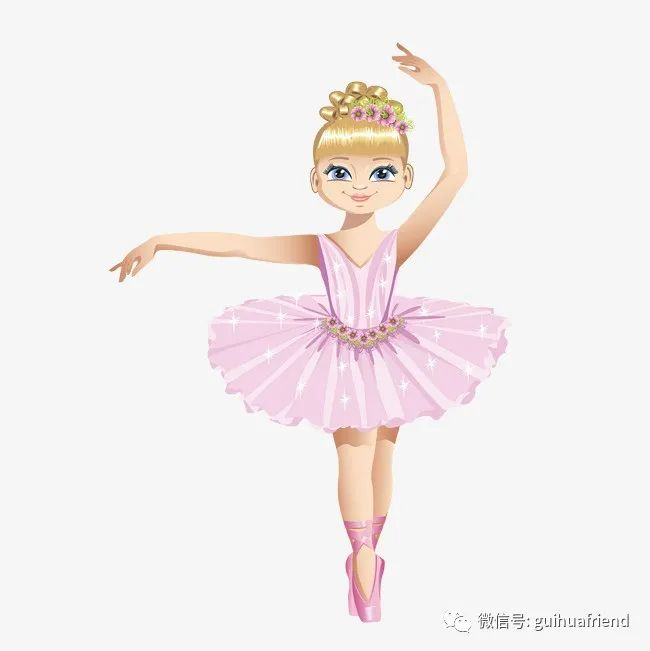
\includegraphics[width = .5\textwidth]{./ch/11.jpg}

\end{figure}



妈妈给我报了一个拉丁舞培训班。

上课的第一天,来到舞蹈学校里,穿上老师为我们准备的舞蹈服装,进了教室。开始,老师先教我们几个动作热身,拉伸。做完后,老师就是开始教基本步,分别有方形步、四分之一转、移动步、朗德追步、前进后退步,定点转和纽约步。

老师耐心的教我们怎么跳?怎么摆,到我们会跳了。老师便放起音乐,嘴里数着节奏:“一二三四,二二三四……”最后跳着步伐加上手的动作完美结合起来。在老师带领下,按照方法努力地练习。顿时,额头已满是汗珠。

接下来,老师又开始教我们第一个组合动作。组合动作都是由一些基本步组成的。老师一个步子一个步子地教,有些同学总跳错,都无精打彩的,通过老师的鼓励,个个都精神起来,经过长时间练习,终于学会了,可高兴了!

无论做什么,只要坚持不懈,就肯定能学会,所以我们学习也要这样。





\vspace{10pt}



作者:四(2)班 徐诗言



指导老师:陈小丽



投稿:2021年6月2日



发表:2021年6月3日








                



\vspace{10pt}

\hline



